\documentclass[11pt, twoside, a4paper]{article}

\usepackage[top=15mm, bottom=15mm, left=25mm, right=25mm]{geometry}
\usepackage{tikz}
\usepackage{amssymb,amsmath, amsthm}
\usepackage[labelsep=period]{caption}

\newtheorem{theorem}{Theorem}[section]
\newtheorem{corollary}{Corollary}[theorem]
\newtheorem{lemma}[theorem]{Lemma}

\newcommand{\Figure}[1]{Figure~\ref{#1}}
\newcommand{\Eq}[1]{Eq.~(\ref{#1})}
\newcommand{\Eqs}[2]{Eqs.~(\ref{#1})--(\ref{#2})}
\newcommand{\set}[1]{\mathbb{#1}}

\begin{document}
\title{Euler 94: Almost equilateral triangles}
\date{}
\author{Didier Pieroux}
\maketitle

-===============================================================================
\begin{abstract} 
-===============================================================================

It is easily proved that no equilateral triangle exists with integral length sides and integral area. However, the almost equilateral triangle 5-5-6 has an area of 12 square units.

We shall define an almost equilateral triangle to be a triangle for which two sides are equal and the third differs by no more than one unit.

Find the sum of the perimeters of all almost equilateral triangles with integral side lengths and area and whose perimeters do not exceed one billion (1,000,000,000).
\end{abstract}

-===============================================================================
\section{Formulation}
-===============================================================================

Let consider an isosceles triangle of base $b\in\set N$, of equal sides $a\in\set N$, and of height $h$ (\Figure{fig:triangle1}).
  
\begin{figure}[h]
    \begin{center}
        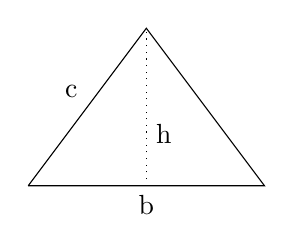
\begin{tikzpicture}[scale=0.5]
        \draw (0, 0) 
           -- (6, 0) node[midway, below] {b} 
           -- (3, 4) 
           -- (0, 0) node[midway, above left] {c} ;
        \draw[dotted] (3, 0) -- (3, 4) node[pos=0.33, right] {h};
        \end{tikzpicture}
        \caption{Geometric description}
        \label{fig:triangle1}
    \end{center}
\end{figure}

The problem is then described by the following equations, with $P$ the perimeter and $S$ the area:
\begin{align}
    c^2 & = (b/2)^2 + h^2 \\ \label{eq:pytha1}
    c & = b \pm 1 \\ \label{eq:ab}
    P & = 2c+b \\ 
    S & = bh/2 \\ \label{eq:S1}
\end{align} 
    
\begin{lemma}$b$ is even.\end{lemma}
\begin{proof} Let suppose that $b$ is odd. For $S$ to be integral, $h$ must be an even integer: $h=2h'$ with $h'\in\set N$. But then $a^2 = b^2/4 + 4h'^2$ is not integral, `which contradicts the hypothesis that $a$ is integral.
\end{proof}

For ease, let us pose $b=2c$ with $c\in\set N$ (\Figure{fig:triangle2}). 
\begin{figure}
    \begin{center}
        \begin{tikzpicture}[scale=0.5]
        \draw          (0, 0) -- (3, 0) node[midway, below] {a};
        \draw [dashed] (3, 0) -- (6, 0) -- (3, 4);
        \draw          (3, 4) -- (0, 0) node[midway, above left] {c} ;
        \draw [dotted] (3, 0) -- (3, 4) node[pos=0.33, right] {h};
        \end{tikzpicture}
        \caption{Reformulated geometric description}
        \label{fig:triangle2}
    \end{center}
\end{figure}

The \Eqs{eq:pytha1}{eq:S1} read now:
\begin{eqnarray}
c^2 & = & a^2 + h^2 \\ \label{eq:pytha2}
  c & = & 2a \pm 1 \\ \label{eq:ac}
  P & = & 2(a+c) \\ 
  S & = & ah \label{eq:S2}
\end{eqnarray}

\Eq{eq:pytha2} shows that $a$, $h$ and $c$ form a Pythagorean triple\footnote{https://en.wikipedia.org/wiki/Pythagorean\_triple}.

\begin{lemma}
	$a$, $h$ and $c$ are pair-wise co-primes. 
\end{lemma}

\begin{proof} 
	Suppose first that $a$ and $c$ are not co-prime, i.e.\ that $\exists\lambda\in\set N$ with $1<\lambda$ such that $a=\lambda a'$ and $c=\lambda c'$. From \Eq{eq:ac}, it then comes $\lambda c = 2 \lambda a \pm 1 \Rightarrow c = 2 a \pm 1/\lambda\ \Rightarrow c \not\in\set N$, which is inconsistent with the integral nature of $c$.
	
	This first result implies that $c$ and $h$ are co-primes. Otherwise, $c$ and $h$ would have a common factor, which should also be a factor of $a$ in order to satisfy \Eq{eq:pytha2}. A similar reasoning shows that $a$ and $h$ must be co-prime.
\end{proof}

This means that $(a, h, c)$ must be a primitive Pythagorean triple.

\section{Tree of primitive Pythagorean triples}
Let consider the infinitely-deep ternary tree whose root is the column vector $p=(3, 4, 5)^T$ and whose child nodes are obtained by left-multiplying their parent by one of the matrices below:
		\[
		A = \left(\begin{matrix}  1 & -2 & 2 \\  2 & -1 & 2 \\  2 & -2 & 3 \end{matrix} \right)\!,\ 
		B = \left(\begin{matrix}  1 &  2 & 2 \\  2 &  1 & 2 \\  2 &  2 & 3 \end{matrix} \right)\!,\
		C = \left(\begin{matrix} -1 &  2 & 2 \\ -2 &  1 & 2 \\ -2 &  2 & 3 \end{matrix} \right)\!.
		\]
Otherwise said, the nodes of the tree are, in breadth-first order:
\[p, Ap, Bp, Cp, AAp, BAp, CAp, ABp, \ldots\] 
It can be shown that this sequence of nodes provides all the primitive Pythagorean triples, and only them, without duplication\footnote{https://en.wikipedia.org/wiki/Tree\_of\_primitive\_Pythagorean\_triples}.

\end{document}
